\documentclass[tikz,border=8pt]{standalone}
\begin{document}
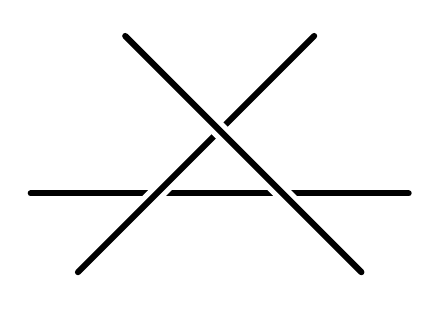
\begin{tikzpicture}[line cap=round,line join=round]
  \tikzset{strand/.style={draw=black,line width=2.2pt,fill=none}}
  % Three pairwise crossings form the triangular region moved by RIII.
  % Drawing order records A below B below C at their crossings.
  \draw[strand] (-2.4,0) -- (2.4,0);
  \draw[white,line width=6pt] (-1.8,-1) -- (1.2,2);
  \draw[strand] (-1.8,-1) -- (1.2,2);
  \draw[white,line width=6pt] (-1.2,2) -- (1.8,-1);
  \draw[strand] (-1.2,2) -- (1.8,-1);
\end{tikzpicture}
\end{document}
